\documentclass[twocolumn,linenumbers]{aastex63}
\usepackage{amsmath}
\usepackage{bm}
\usepackage{xspace}
\newcommand{\photoz}{photo-$z$\xspace}
\newcommand{\cosmos}{COSMOS2020\xspace}
\newcommand{\given}{\,|\,}
% Generated by analysis/build_apjl_assets.py; do not edit numerical values here.
\newcommand{\NParent}{162,239}
\newcommand{\NTrain}{111,952}
\newcommand{\NValidation}{23,652}
\newcommand{\NPhotTest}{26,635}
\newcommand{\NTest}{5,083}
\newcommand{\FlowScatter}{0.0178}
\newcommand{\SpecScatter}{0.0210}
\newcommand{\MatchedScatter}{0.0220}
\newcommand{\ScatterGainSpec}{15}
\newcommand{\ScatterGainEazy}{37}
\newcommand{\OutlierGainEazy}{72}

\shorttitle{Distilling COSMOS Redshift Posteriors}
\shortauthors{Working draft}
\hypersetup{
  pdftitle={Distilling COSMOS2020 Redshift Posteriors into Broadband Normalizing Flows},
  pdfauthor={},
  pdfsubject={ApJL-style working draft: COSMOS posterior transfer experiment},
  pdfkeywords={photometric redshifts, COSMOS2020, normalizing flows}
}
\let\originalbibliography\thebibliography
\renewcommand{\thebibliography}[1]{%
  \originalbibliography{#1}%
  \setlength{\itemsep}{0pt}%
  \setlength{\parsep}{0pt}%
  \setlength{\parskip}{0pt}%
  \setlength{\bibsep}{0pt}%
  \raggedright
}

\begin{document}
\title{Distilling COSMOS2020 Redshift Posteriors into Broadband Normalizing Flows}
% Author names and affiliations intentionally omitted at the author's request.
% Author names, affiliations, ORCIDs and correspondence information are unset.
% Add \author and \affiliation commands here when the author list is agreed.


\begin{abstract}
Deep multiband photometric redshifts can extend broadband training beyond
available spectroscopy if their uncertainties are propagated.
We present a framework that samples redshift labels from released
COSMOS2020 LePhare distributions and trains a conditional normalizing flow.
We select \NParent\ galaxies with HSC $i<25$ in $2''$ apertures and add
noise to native CFHT $u$/HSC $grizy$ measurements to approximate LSST
ten-year depths. On \NTest\ held-out spectroscopic galaxies, the flow
trained on \NTrain\ probabilistic labels achieves
$\sigma_{\rm NMAD}=\FlowScatter$, compared with \SpecScatter\ for a broadband
flow trained on 22,604 spectroscopic labels. It also has lower scatter
than the adopted six-band EAZY benchmark. Full-multiband LePhare remains
more accurate, but its nominal 68\% intervals contain only 56.3\% of test
redshifts, compared with 68.6\% for the bootstrapped flow.
The flow comparison changes both training size and selection, and the
test sample is spectroscopically selected. These results demonstrate
probabilistic redshift transfer; they do not establish calibration for
the full photometric population or measured Rubin photometry.
\end{abstract}
\keywords{Photometric redshift --- Astrostatistics --- Galaxy surveys}

\section{Introduction}\label{sec:intro}
Photometric redshifts (photo-$z$s) enable studies of galaxy evolution and
cosmology with millions to billions of galaxies. They provide distances
for tracing galaxy populations and mapping the matter distribution with
weak gravitational lensing. Photo-$z$ errors, however, already limit
cosmological analyses. In the Hyper Suprime-Cam (HSC) Year-3 joint
clustering and weak-lensing analysis, accounting for residual photo-$z$
uncertainty lowered the inferred $S_8=\sigma_8\sqrt{\Omega_m/0.3}$ from
$0.791^{+0.018}_{-0.020}$ to $0.763^{+0.040}_{-0.036}$ and roughly doubled
its error bars \citep{miyatake2023,hahn2024}. Current photo-$z$s also exhibit
biases and underestimated uncertainties. Even COSMOS2020, which uses deep
multiband imaging, shows magnitude-dependent biases and apparent
overconfidence for faint galaxies in spectroscopic comparisons
\citep{weaver2022}.

Photo-$z$ calibration will be more demanding for the Vera C.~Rubin
Observatory's Legacy Survey of Space and Time \citep[LSST;][]{ivezic2019}.
LSST will image approximately $18{,}000\,\mathrm{deg}^2$ in six broadband
filters, $ugrizy$, over ten years and is expected to observe approximately
20 billion galaxies. Exploiting this statistical power requires accurate
redshift distributions for the galaxies used in cosmological analyses
\citep{desc2018}. Calibration data that reach the depth and span the galaxy
populations of LSST will be a major bottleneck.

Secure spectroscopic redshifts provide the reference standard for photo-$z$
training and calibration. DESI achieves redshift precisions of approximately
$10$--$40\,\mathrm{km\,s^{-1}}$ for its main galaxy samples \citep{lan2023}.
These errors are negligible compared with broadband photo-$z$ uncertainties,
so reliable spectroscopic measurements can be treated as known labels.
Self-organizing-map methods group galaxies with similar photometry and use
reference redshifts to calibrate their redshift distributions. SOMPZ connects
these groups in deep and wide-field photometry to infer tomographic redshift
distributions \citep{buchs2019,myles2021}. In DES, its reference sample
combines spectroscopy with high-quality multiband photo-$z$s.

The main limitation of spectroscopic calibration is selection. Spectroscopic
samples preferentially contain brighter galaxies and objects with identifiable
spectral features. Photo-$z$ estimators trained on these samples can therefore
inherit their selection biases. Restricting analyses to galaxies represented
by spectroscopy reduces this risk but discards statistical power. The
KiDS-1000 SOM-gold selection, for example, reduced the effective source density
by approximately 20\% \citep{hildebrandt2021,giblin2021}. Obtaining
representative spectroscopy at LSST depths would require substantial telescope
time. \citet{newman2015} estimate that conventional training requires at least
approximately 30,000 spectra across multiple independent fields, reaching
the faint limits of the science sample.

Deep multiband imaging offers an alternative. COSMOS2020 combines more than
30 photometric bands across approximately $2\,\mathrm{deg}^2$, including
12 optical intermediate bands and two narrow bands \citep{weaver2022}.
These measurements constrain redshift more precisely than broadband photometry
alone: normalized redshift scatter is below 1\% for $i<21$ galaxies and
reaches approximately 5\% at $25<i<27$. These photo-$z$s cannot be treated
as exact labels. Their released redshift probability distributions, however,
allow us to propagate their uncertainties into a broadband estimator.
Their calibration must also be tested: \citet{weaver2022} find underestimated
uncertainties at faint magnitudes, while noting that spectroscopic selection
complicates this comparison.

In this work, we present a framework that propagates deep multiband redshift
uncertainties into broadband photo-$z$s using normalizing flows. We sample
redshifts from the deep-field probability distributions and broadband
measurements from a photometric transfer model, then train a conditional flow
on these samples. Normalizing flows can represent complex, multimodal
distributions and provide efficient likelihood evaluation and sampling
\citep{durkan2019,papamakarios2021}. Under a conditional sufficiency assumption,
this procedure marginalizes over the deep observations to estimate
$p(z\given x)$ for broadband measurements $x$. It propagates the input
redshift uncertainties but does not automatically correct their systematic
errors.

We demonstrate this framework with public COSMOS2020 data. We use the released
multiband redshift distributions to train a flow on CFHT $u$/HSC $grizy$
photometry, adding noise where needed to approximate LSST ten-year depths.
The experiment retains the native COSMOS filters and uses an explicit noise
model for the transfer. On a spatially held-out spectroscopic sample, we
compare our predictions with a spectroscopically trained broadband flow,
broadband template fitting, and full-multiband template-fitting estimates.
We test both redshift accuracy and uncertainty calibration to assess whether
probabilistic labels can extend broadband training to larger and fainter
samples.

\section{Observations}\label{sec:observations}
\subsection{COSMOS2020}
We use the \cosmos Classic catalog and its released LePhare v2.1 redshift
probability distributions \citep{weaver2022,ilbert2006}. We select galaxies
with \texttt{flag\_combined}=0, \texttt{lp\_type}=0, HSC $i_{\rm ap}<25$ AB
in a $2''$ aperture, and native $i$-band signal-to-noise ratio $\geq5$.
We require finite CFHT $u$/HSC $grizy$ fluxes, positive flux uncertainties,
and a finite, nonnegative redshift PDF with nonzero integral. Negative fluxes
outside the $i$ band are retained. Of 170,003 objects passing the magnitude
and signal-to-noise cuts, \NParent\ have usable six-band measurements;
all have valid PDFs. Selection does not require spectroscopy.

We divide the field into $0.05^\circ$ sky cells and randomly assign cells
to training, validation, and test sets with probabilities 0.70, 0.15, and
0.15, using seed 20261024. We fix these assignments before magnitude
selection. The resulting sets contain \NTrain, \NValidation, and
\NPhotTest\ galaxies. No galaxy in a test cell is used for training.

\subsection{LSST-like Broadband Photometry}
The deep COSMOS observations provide both the multiband redshift labels and
the broadband measurements used to train our estimator. Using their native
broadband precision would test performance at COSMOS depth, rather than at
the noise levels expected for LSST. Photometric noise broadens color--redshift
degeneracies and changes the conditional distribution $p(z\given x)$.
We therefore add noise to the broadband inputs while retaining the redshift
information from the deep multiband observations. This lets us test how well
that information transfers to noisier broadband measurements and evaluate
all broadband methods on the same inputs.

We use native CFHT $u$ and HSC $grizy$ aperture measurements and add noise
to approximate LSST ten-year depths. The adopted $5\sigma$ point-source
depths are $(25.6,26.9,26.9,26.4,25.6,24.8)$ AB \citep{rubindepths}.
For each band, we set
\begin{align}
\sigma_{\rm tar}&=\frac{10^{(23.9-m_5)/2.5}}{5}\ \mu{\rm Jy},\\
\sigma_{\rm eff}&=\max(\sigma_{\rm deep},\sigma_{\rm tar}),\\
f'&=f_{\rm deep}+\epsilon,\quad
\epsilon\sim\mathcal N(0,\sigma_{\rm eff}^2-\sigma_{\rm deep}^2).
\label{eq:kernel}
\end{align}
We draw noise independently between bands and retain measurements already
noisier than the target depth. Selection precedes noise addition.
This model changes the noise level but retains the native filters.
It does not reproduce Rubin bandpasses, detection, blending, or correlated
measurement errors.

\subsection{Spectroscopic Redshifts}
We match Classic identifiers to the DR1.1 unique-object COSMOS spectroscopic
compilation \citep{khostovan2025}. We retain public galaxy measurements with
quality flags 3, 4, 13, or 14 and positive finite spectroscopic redshifts.
The parent match also requires a valid nonnegative catalog photo-$z$.
For duplicate observations, we use the compilation's preferred measurement.
We impose no photo-$z$/spec-$z$ agreement cut. The labels combine programs
including DESI, zCOSMOS, DEIMOS, C3R2, and LEGA-C.

The training, validation, and test sets contain 22,604, 4,803, and \NTest\
secure spectroscopic matches. We evaluate all methods on these same
\NTest\ test galaxies. Spectroscopy strongly favors brighter objects:
the median $i_{\rm ap}$ is 22.69 for the spectroscopic test sample and
24.17 for the full photometric test sample. Appendix~\ref{sec:selection}
shows their magnitude distributions.

\subsection{Benchmark Photo-zs}
We compare our method with three benchmarks:
\begin{itemize}
\item \textbf{Broadband flow.} A conditional flow trained on secure
spectroscopic redshifts. It uses the same architecture, six-band inputs,
preprocessing, noise augmentation, optimizer, and stopping rules as our
method. Only the training population and redshift labels differ.
We use this benchmark instead of SOMPZ because it directly compares
individual conditional redshift distributions within one model family.
SOMPZ groups galaxies in photometric space to calibrate ensemble redshift
distributions \citep{buchs2019,myles2021}. The flow avoids this discretization
and isolates differences from training data without introducing a different
estimator. We do not test whether it outperforms SOMPZ.

\item \textbf{Broadband EAZY.} Template fitting with EAZY-py 0.8.7
\citep{brammer2008}. We fit the saved noisy test measurements using its
12 tweaked FSPS templates, nonnegative template coefficients, 1\% systematic
flux error, and template-error amplitude 0.20. The redshift grid spans
$0.001<z<10$ with $\Delta z/(1+z)=0.005$. We correct fluxes and errors for
catalog Galactic extinction and apply the supplied
\texttt{prior\_R\_zmax7.dat} to HSC $r$, with an aperture-to-total correction.
This filter mapping is approximate. We fit no population-specific prior,
zero-point, or template corrections and provide no test redshifts to EAZY.

\item \textbf{Full-multiband LePhare.} The released COSMOS2020 redshift
distribution.
It supplies our training labels and uses more photometric information than
the broadband methods. Its comparison measures how much accuracy is retained
when transferring to six noisy bands.
\end{itemize}
Both template-fitting benchmarks have calibration histories that differ
from those of our flows.

\section{Bootstrapping Narrowband Photo-z}\label{sec:bootstrapping}
We use deep multiband redshift distributions as probabilistic training labels.
Here, ``narrowband'' refers to the full COSMOS photometry, including its
intermediate and narrow bands. ``Bootstrapping'' denotes transferring this
redshift information to broadband measurements; it is distinct from the
bootstrap resampling used to estimate statistical errors below.

Figure~\ref{fig:workflow} summarizes training. Deep multiband
redshift PDFs are needed only during training; inference uses broadband
fluxes and their uncertainties.

\begin{figure*}[t]
\centering
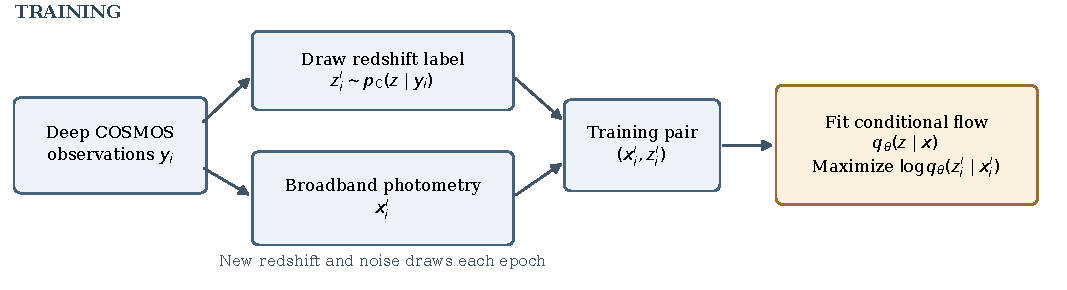
\includegraphics[width=\textwidth]{figures/fig05_bootstrap_workflow.pdf}
\caption{\label{fig:workflow}
Workflow of the bootstrapped flow. For each training galaxy, we independently
draw a redshift from its released COSMOS2020 PDF and a noisy broadband
measurement conditional on its deep observations. We fit the conditional
flow to these pairs, drawing new labels and noise each epoch.
The photometric transfer uses the explicit noise model
in Equation~\ref{eq:kernel}; the input redshift PDFs are not recalibrated.}
\end{figure*}

Let $y$ denote the deep observations, $z$ redshift, and
$x=(\bm f,\bm\sigma)$ the broadband fluxes and uncertainties.
For the selected COSMOS population $S$, we assume $z\perp x\given y,S$.
If the released distribution $p_{\rm C}(z\given y)$ describes the true
conditional redshift distribution, then
\begin{equation}
p(z\given x,S)=\int p_{\rm C}(z\given y)\,p(y\given x,S)\,dy.
\label{eq:target}
\end{equation}
We approximate this integral by sampling redshifts from the released PDFs
and broadband measurements from the noise model $K(x\given y)$ in
Equation~\ref{eq:kernel}. We train a conditional normalizing flow
$q_\theta(z\given x)$ by minimizing
\begin{equation}
\mathcal L(\theta)=-\frac{1}{N}\sum_i
\mathbb E_{\substack{z\sim p_{\rm C}(z\given y_i)\\
                    x\sim K(x\given y_i)}}
\left[\log q_\theta(z\given x)\right].
\label{eq:loss}
\end{equation}
We draw a new redshift and new photometric noise for each galaxy at each
training traversal. These draws are independent conditional on $y_i$.
We normalize the released PDFs over $0\leq z\leq10$, interpolate their
densities linearly between grid points ($\Delta z=0.01$), and sample by
inverting the continuous cumulative distribution. We apply no recalibration
to the input PDFs. We call this estimator the \emph{bootstrapped flow}.

Equation~\ref{eq:loss} fits the conditional distribution defined by the
input PDFs, photometric population, and noise model. It therefore propagates
any errors or prior dependence in those PDFs. We do not divide the labels
by a global $p(z)$: our target is a conditional redshift distribution for
$S$, not a redshift likelihood. Applying the model to another population
requires checking population coverage and selection. This experiment tests
neither the sufficiency assumption nor the correctness of the input PDFs.

The flow uses two conditional rational-quadratic spline transforms, each
with 16 bins, hidden width 64, and two residual blocks, with a standard-normal
base \citep{durkan2019}. We transform redshift as
$t=\{\log[z/(10-z)]+2.2\}/1.1$ and include its Jacobian in the density.
Inputs are six asinh-transformed fluxes with softening $0.02\,\mu$Jy and
six log uncertainties. We estimate feature normalization from the full
photometric training set.

We train with AdamW, learning rate $8\times10^{-4}$, batches of 512,
and gradient clipping at 5. We allow at most 200 epochs and 20,000 steps,
with validation-based learning-rate reduction and early stopping.
The bootstrapped flow uses fixed posterior draws for validation; the
broadband flow uses spectroscopic labels. They train for 20,000 and
7,515 steps, respectively. We use one training seed for each model.

\section{Results}\label{sec:results}
\subsection{Redshift Accuracy}
We compare four methods on the same \NTest\ held-out spectroscopic galaxies
(Table~\ref{tab:results}). For each method, we use the posterior median
$z_{50}$ as the point estimate and define the normalized residual
$r=(z_{50}-z_{\rm spec})/(1+z_{\rm spec})$. We report the median bias
$b={\rm median}(r)$, robust scatter
$\sigma_{\rm NMAD}=1.4826\,{\rm median}|r-b|$, and outlier fraction
$\eta=P(|r|>0.15)$.

\begin{deluxetable*}{lrrrrrr}
\tablecaption{Performance on the same 5,083 held-out spectroscopic galaxies.\label{tab:results}}
\tablewidth{0pt}
\tablehead{\colhead{Method} & \colhead{$N_{\rm train}$} & \colhead{$b$} & \colhead{$\sigma_{\rm NMAD}$} & \colhead{$\eta$ (\%)} & \colhead{$C_{68}$ (\%)} & \colhead{$C_{95}$ (\%)}}
\startdata
Bootstrapped flow & 111,952 & -0.0064 & 0.0178 & 2.81 & 68.6 & 94.7 \\
Broadband flow & 22,604 & +0.0001 & 0.0210 & 3.07 & 66.0 & 94.0 \\
EAZY, supplied R prior & \nodata & -0.0017 & 0.0285 & 10.11 & 59.9 & 85.6 \\
LePhare, full COSMOS & \nodata & -0.0028 & 0.0100 & 2.30 & 56.3 & 82.0 \\
\enddata
\tablecomments{All point estimates are posterior medians; $C_\alpha$ is equal-tailed interval coverage. The first three methods use six broadband measurements at inference; released LePhare uses the full deep COSMOS photometry and is the training teacher. EAZY is not calibrated on this population. An ellipsis indicates no training set fitted in this experiment, not absence of prior calibration in the released methods.}
\end{deluxetable*}


The bootstrapped flow achieves $\sigma_{\rm NMAD}=\FlowScatter$, compared
with \SpecScatter\ for the broadband flow: a \ScatterGainSpec\% reduction.
The paired-bootstrap 95\% interval for the scatter difference is
$[-0.0040,-0.0024]$. Its outlier fraction is 2.81\%, compared with 3.07\%
for the broadband flow. This difference is not significant: its 95\%
interval spans $[-0.55,+0.08]$ percentage points. The bootstrapped flow also
has a larger absolute bias ($-0.0064$ versus $+0.0001$) and normalized
root-mean-square residual (0.158 versus 0.151). Its advantage is in robust
scatter, not every accuracy measure. The flows differ in both training
sample size and selection; this comparison does not separate these effects.

\begin{figure*}[!t]
\centering
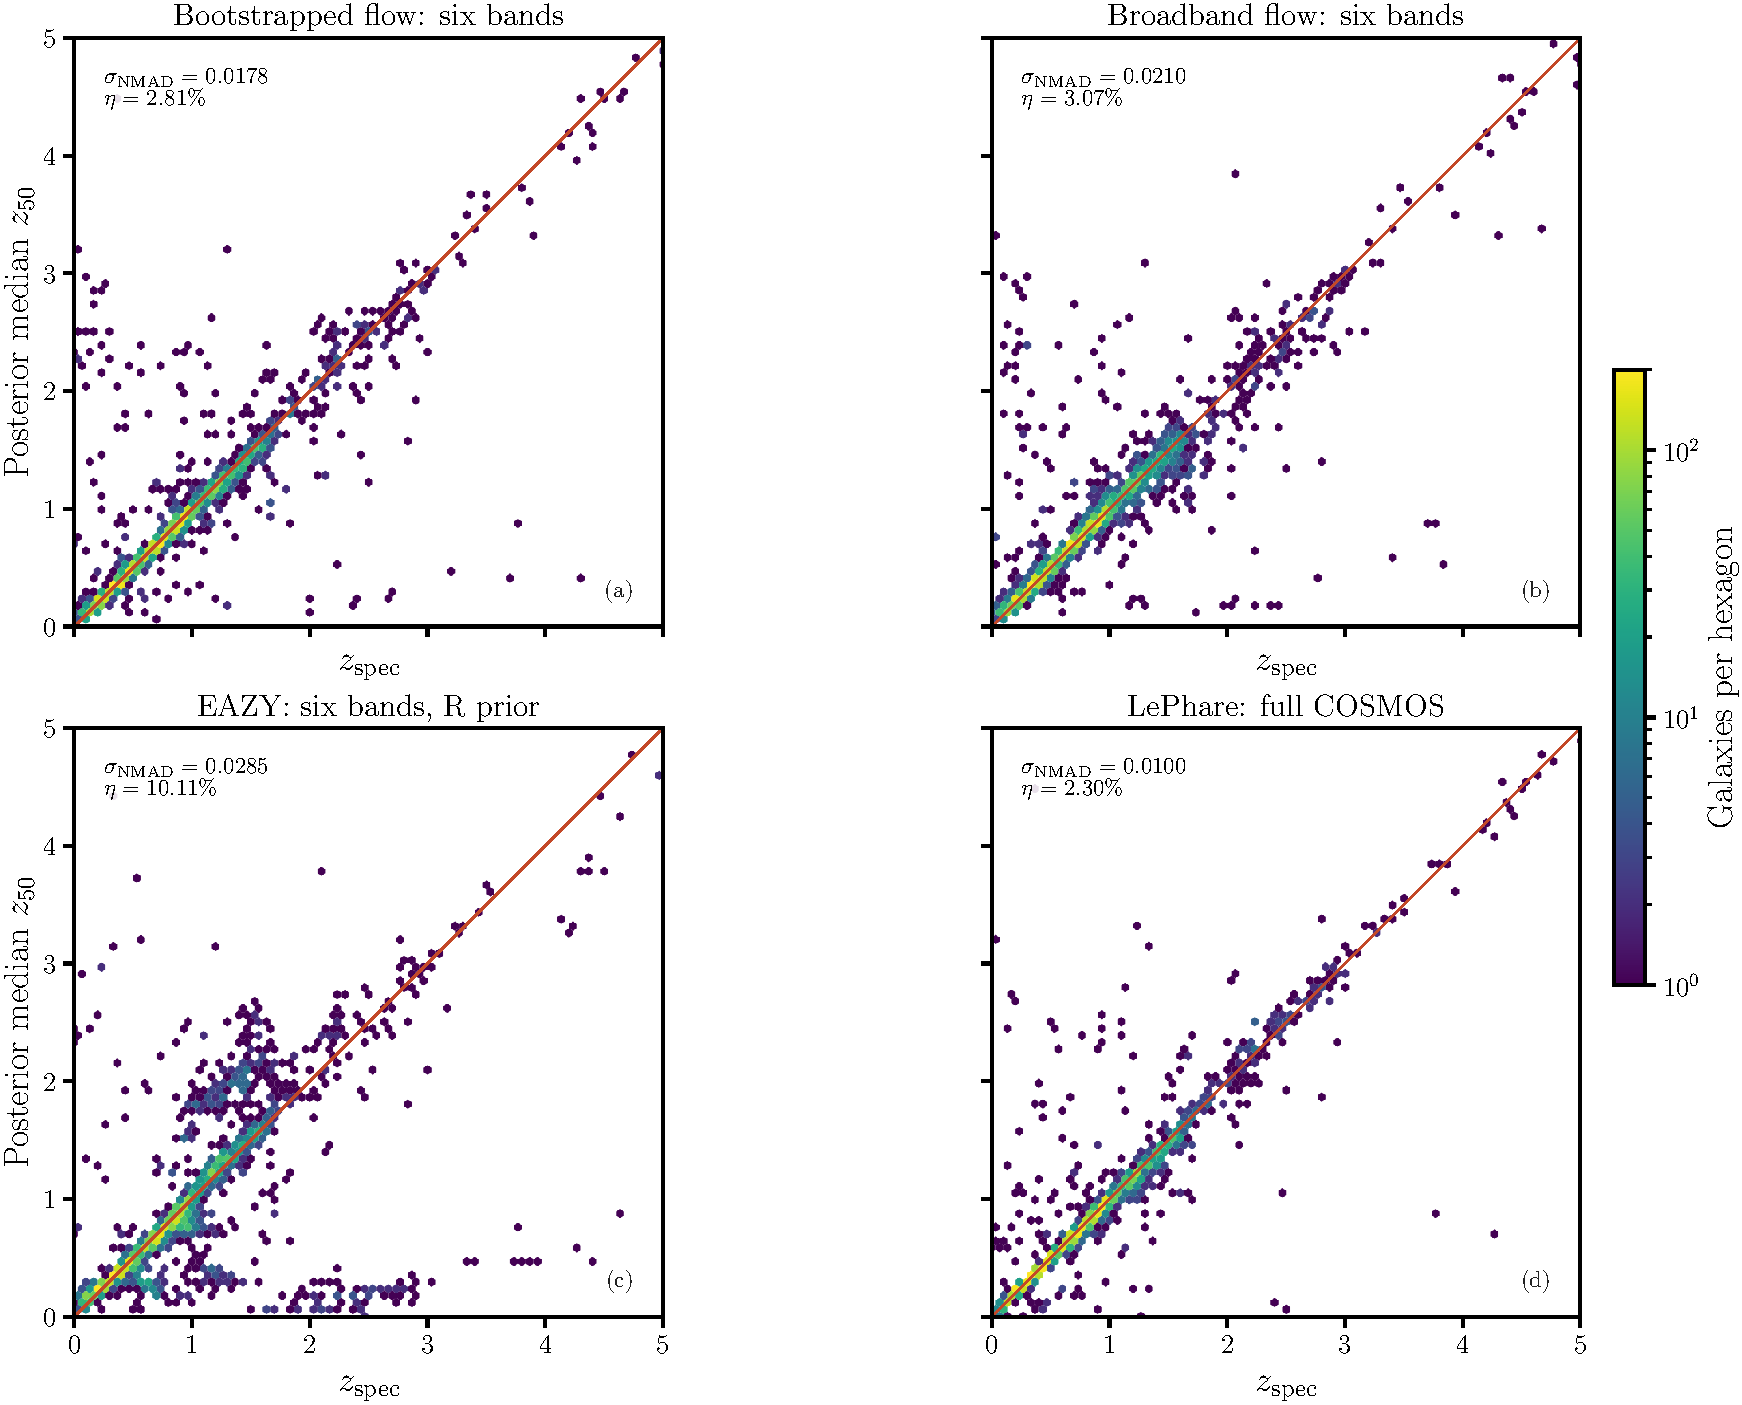
\includegraphics[width=\textwidth,height=0.48\textheight,keepaspectratio]{figures/fig02_accuracy.pdf}
\caption{\label{fig:accuracy}
Posterior-median redshifts for the bootstrapped and broadband flows, EAZY with
its supplied R prior, and full-multiband LePhare, evaluated on the same
\NTest\ galaxies. Colors show counts per hexagon on a shared logarithmic
scale. The diagonal marks equality. Panels show $z<5$; statistics include
the full test sample. LePhare uses the full deep photometry and supplies
the bootstrapped flow's training labels.}
\end{figure*}

Figure~\ref{fig:accuracy} compares the bootstrapped flow with template fitting.
Broadband EAZY gives scatter 0.0285 and 10.11\% outliers. The bootstrapped
flow has \ScatterGainEazy\% lower scatter and \OutlierGainEazy\% fewer
outliers. EAZY is not calibrated on this population, whereas the flow learns
from \NTrain\ probabilistic labels. The comparison therefore applies to
this EAZY configuration, not an optimized template-fitting pipeline.
Using EAZY's posterior mode instead of its median gives scatter 0.0326
and 12.02\% outliers and does not reverse the comparison.

Full-multiband LePhare gives lower scatter (0.0100) and fewer outliers
(2.30\%) than the bootstrapped flow. Its catalog point estimates give
nearly identical results to the PDF medians. This is consistent with the
additional information in the deep multiband measurements, although we
cannot separate information loss from approximation errors in the flow.

\subsection{Uncertainty Calibration}
We measure equal-tailed interval coverage,
\begin{equation}
C_\alpha=\frac{1}{N}\sum_i
\mathbf1\left\{\frac{1-\alpha}{2}\leq
F_i(z_{{\rm spec},i})\leq\frac{1+\alpha}{2}\right\},
\end{equation}
where $F_i$ is the predicted cumulative redshift distribution.
For representative draws from a calibrated model, $C_\alpha=\alpha$.
Our spectroscopic test sample is selected, so coverage here need not
represent the full photometric population.

\begin{figure}[!htbp]
\centering
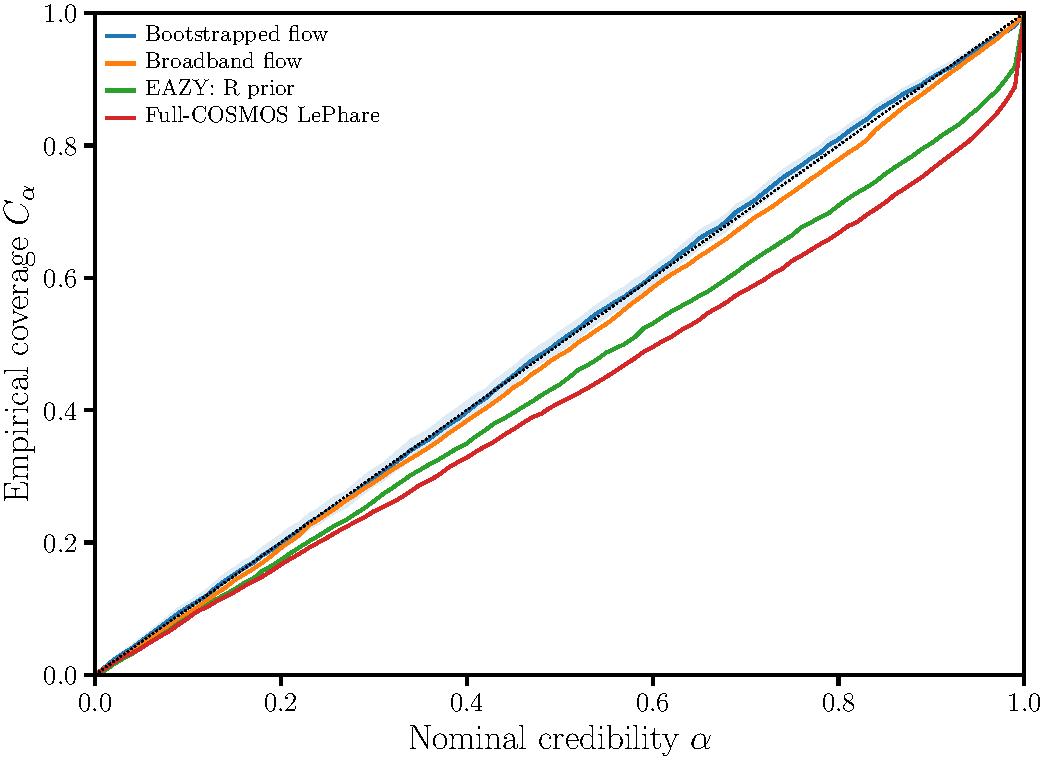
\includegraphics[width=\columnwidth]{figures/fig03_calibration.pdf}
\caption{\label{fig:calibration}
Equal-tailed interval coverage on the common spectroscopic test sample.
The dotted diagonal marks nominal coverage. Shading shows the bootstrapped
flow's 95\% pointwise galaxy-bootstrap interval. Agreement with the diagonal
on this selected sample does not establish population-wide calibration.}
\end{figure}

The bootstrapped flow's nominal 68\% and 95\% intervals contain 68.6\%
and 94.7\% of test redshifts (Figure~\ref{fig:calibration}). The broadband
flow gives 66.0\% and 94.0\%, broadband EAZY gives 59.9\% and 85.6\%,
and full-multiband LePhare gives 56.3\% and 82.0\%.
The median 68\% interval width is 0.0643 for the bootstrapped flow and
0.0259 for LePhare. The bootstrapped flow nevertheless has an asymmetric
probability integral transform, $F_i(z_{{\rm spec},i})$, consistent with
its residual bias. Nearly nominal central coverage can hide unequal tail
errors. Broader intervals after transfer do not demonstrate that the flow
corrects errors in its training PDFs.

We also evaluate LePhare on 34,792 secure spectroscopic matches without
the $i<25$ cut. Its 68\% and 95\% intervals contain 55.7\% and 81.8\%
of redshifts. We apply TARP \citep{lemos2023}, which measures PDF mass
within $|z_{\rm spec}-r_0|$ of a random reference $r_0$. We draw 64 references
per galaxy, either uniformly over $[0,10]$ or within $0.25(1+z_{50})$ of
the median, clipped to the PDF support. The global and local TARP curves
differ, indicating that a single width correction may be insufficient.
The undercoverage agrees qualitatively with \citet{weaver2022}, who report
underestimated faint-galaxy uncertainties. Their sample and interval
definition differ from ours, and spectroscopic selection may contribute
to both results. Undercoverage alone does not establish redshift bias.

We estimate 95\% intervals by resampling galaxies: 200 paired resamples for
the flow comparison and magnitude bins, and 300 for template comparisons
and the coverage band. These intervals exclude training variance, spatial
covariance, and uncertainty from spectroscopic selection. Synthetic
calibrated and narrowed-PDF controls, CDF-inversion checks, and
comparisons of direct and cached EAZY outputs verify the numerical procedure.

\subsection{Magnitude Dependence}
\begin{figure}[!htbp]
\centering
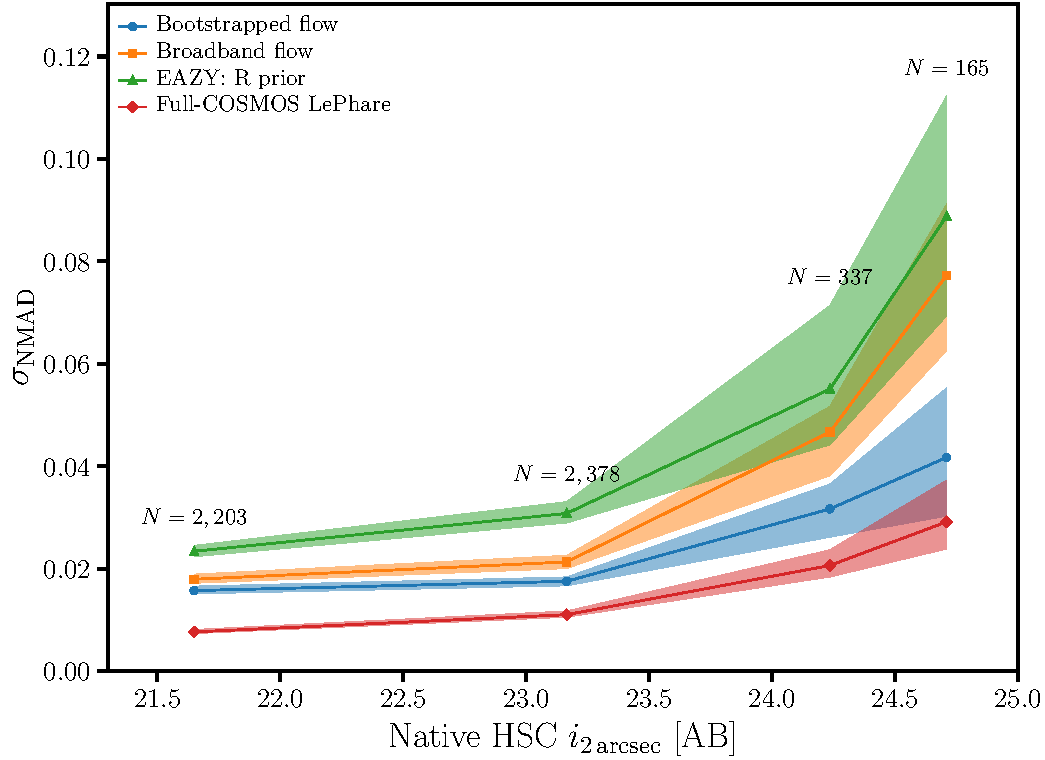
\includegraphics[width=\columnwidth]{figures/fig04_magnitude_dependence.pdf}
\caption{\label{fig:magnitude}
Robust redshift scatter versus native, pre-noise HSC $i$ aperture magnitude.
Points lie at the median magnitude of the test galaxies in each bin, with
identical x-coordinates for all methods. The bins $i<22.5$, $22.5\leq i<24$,
$24\leq i<24.5$, and $24.5\leq i<25$ contain 2,203, 2,378, 337, and 165
galaxies, respectively.
Text labels give the galaxy counts. Shaded bands join the 95\% pointwise
galaxy-bootstrap interval endpoints from 200 resamples.
The faint bins sample the available spectroscopy, not the full photometric
population.}
\end{figure}
Figure~\ref{fig:magnitude} compares scatter in magnitude bins. The
bootstrapped flow has lower scatter than the broadband flow, particularly
in the faint bins. However, only 2.35\% of selected photometric objects at
$24.5\leq i_{\rm ap}<25$ have qualifying spectroscopy, and only 165 enter
the test set. The faint-end comparison therefore remains limited by
spectroscopic selection.

At $z_{\rm spec}>2$, the test sample contains 167 galaxies. The bootstrapped
and broadband flows have nearly identical scatter, 0.0547 and 0.0544,
respectively. Their 68\% coverages are 63.5\% and 70.7\%.
Coverage within true-redshift bins need not be nominal even for a calibrated
posterior. Redshift, magnitude, and spectroscopic selection also covary,
so the aggregate improvement does not establish a high-redshift advantage.

\section{Discussion and Conclusions}\label{sec:discussion}
We present a framework for training broadband redshift distributions with
uncertain labels from deep multiband imaging. Applied to COSMOS2020, the
bootstrapped flow has lower robust scatter than a spectroscopically trained
broadband flow and the adopted EAZY configuration. Its nominal intervals
also have nearly correct aggregate coverage on the spectroscopic test
sample. The comparison with the broadband flow changes both training
sample size and selection, so it does not identify which drives the gain.

The method propagates the input PDFs; it does not guarantee their accuracy.
LePhare undercovers in both spectroscopic assessments and has nonzero median
residuals. The bootstrapped flow can inherit template errors, prior dependence,
and missing populations. Its improved aggregate coverage does not show that
these errors are removed. Spatially disjoint splits prevent reuse of test
objects in flow training, but spectroscopy may have contributed to the
original COSMOS template and zero-point calibration. One field also cannot
measure field-to-field population variation.

Our noise-degradation experiment approximates LSST depth, not LSST selection.
DESC gold forecasts adopt $i<24.1$ for Year~1 and $i<25.3$ for Year~10,
using CModel magnitudes and separate weak-lensing selection criteria
\citep{desc2018}. Our $2''$ aperture cut differs: near its boundary, the
median aperture-to-total offset is $-0.22$ mag, corresponding to
$i_{\rm total}\simeq24.78$ at $i_{\rm ap}=25$, before Galactic correction.
We also select galaxies before noise addition and require six usable deep
measurements and a valid redshift PDF. Noise addition does not reproduce
Rubin detection, blending, morphology, or shape selection.

The next step is to test the transfer with matched Rubin and COSMOS
measurements, apply the target selection after transfer, and validate
population coverage. Multiple training seeds, additional deep fields,
and independent faint-galaxy spectroscopy are needed to quantify training
variance, field variation, and selection effects. Recalibration of the
input PDFs should be tested separately. These steps will determine whether
bootstrapping deep multiband redshifts can meet LSST calibration requirements.


\section*{Data and Software Availability}
The draft includes four executable figure notebooks, compact data snapshots,
numerical results, and source-file hashes.
The notebooks reproduce the figures without model retraining or network access.
The underlying photometry and redshift PDFs are available from
\href{https://irsa.ipac.caltech.edu/data/COSMOS/tables/cosmos2020/}{IRSA},
and the spectroscopic compilation from its
\href{https://github.com/cosmosastro/speczcompilation}{public repository}.
We use NumPy, Astropy, Matplotlib, PyTorch, \texttt{nflows}, and
EAZY-py; exact analysis and notebook dependencies are recorded with the code.
EAZY templates and filter responses are credited to their
\href{https://github.com/gbrammer/eazy-photoz}{public repository}.

\clearpage
\appendix
\section{Magnitude Distributions}\label{sec:selection}
Figure~\ref{fig:selection} compares the photometric training population
with the spectroscopic training and test samples. Spectroscopy favors
brighter galaxies even though the photometric selection does not require
a spectroscopic redshift. The test metrics therefore describe the
spectroscopic subset of our magnitude-limited population.

\begin{figure}[ht]
\centering
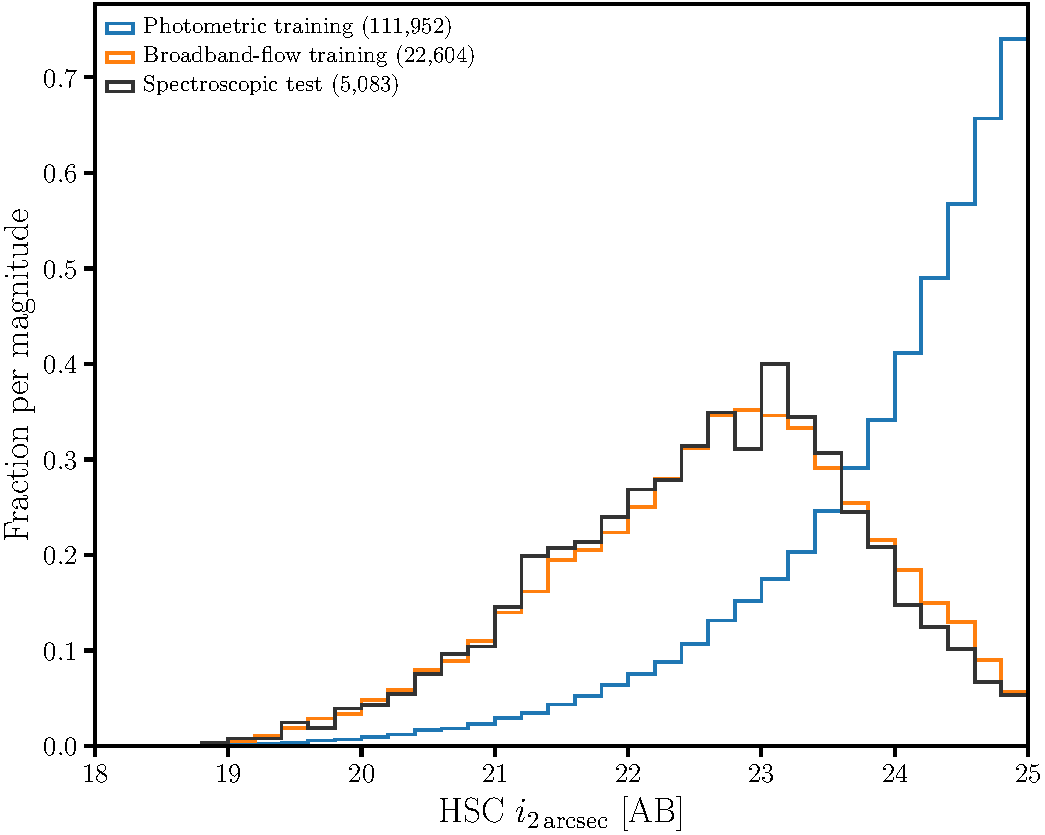
\includegraphics[width=0.55\textwidth]{figures/fig01_selection.pdf}
\caption{\label{fig:selection}
Native HSC $i$-band aperture magnitudes for the full photometric training
sample, broadband-flow spectroscopic training sample, and spectroscopic
test sample. Histograms are normalized separately. The displayed
$18<i<25$ range imposes no additional bright cut.}
\end{figure}


\bibliography{references}
\end{document}
